\documentclass[12pt,letterpaper, onecolumn]{exam}
\usepackage{amsmath}
\usepackage{amsthm}
\usepackage{bm}
\usepackage{amssymb}
\usepackage{tikz}
\usepackage{graphicx}
\usepackage[lmargin=71pt, tmargin=1.2in]{geometry}  % For centering solution box
% \chead{\hline} % Un-comment to draw line below header
\thispagestyle{empty}   % For removing header/footer from page 1

\begin{document}

\begingroup  
    \centering
    \LARGE {\textbf{Probabilistic Techniques and Randomized Algorithms}\\
    \LARGE \textbf{Homework 2024 - 2025}\\
    \large Elective Course - CEID\_NE5017\\[0.5em]
    \large \today\\[0.5em]
    \large \textbf{Professor}: Sotiris Nikoletseas\\[0.5em]
    \large \textbf{Students}: Chrysavgi Pateli, Miltiadis Mantes\par
    \large \textbf{Register numbers}: 1084513, 1084661\par
    \large \textbf{E-mails}: up1084513@ac.upatras.gr, up1084661@ac.upatras.gr\par
\endgroup
\rule{\textwidth}{0.4pt}
\pointsdroppedatright   % Self-explanatory
\printanswers
\renewcommand{\solutiontitle}{\noindent\textbf{Ans:}\enspace}   % Replace "Ans:" with starting keyword in solution box

\begin{questions}

    \question Provide the sample points of the \( G_{3, 1/3} \)
    sample space and the probability of each point.\droppoints
    
    \begin{solution}
    
        In the \( G_{n,p} \) random graph model, we have \( 2^{\binom{n}{2}} \) different random graphs in our sample space, each of which has \( n \) vertices. For each pair of vertices \( (u, v) \), we toss a coin and with probability \( p \) we connect the vertices with an edge, while with probability \( 1-p \) we don't connect them. 
        
        In our case we have random graphs with \( n = 3 \) vertices and the probability that a vertex is connected with another vertex is \( p = \frac{1}{3} \), while the probability that a vertex is not connected with another vertex is \( q = 1-p = \frac{2}{3} \). The total number of possible edges is \( \binom{3}{2} = 3 \), and each edge can either exist (\( 1 \)) or not exist (\( 0 \)). This results in a sample space that contains \( 2^3 = 8 \) possible graphs.

        Below are the sample points, their probabilities, and their visual representations:

        \begin{itemize}
            \item \textbf{Graph 1:} \( (0, 0, 0) \), no vertices are connected, probability \( \bm{P = \left(\frac{2}{3}\right)^3 = \frac{8}{27}} \).
            \begin{center}
                \begin{tikzpicture}
                    \node[circle, draw, fill=black, inner sep=2pt, label=above:\(v_1\)] (A) at (0, 1) {};
                    \node[circle, draw, fill=black, inner sep=2pt, label=below left:\(v_2\)] (B) at (-1, -1) {};
                    \node[circle, draw, fill=black, inner sep=2pt, label=below right:\(v_3\)] (C) at (1, -1) {};
                \end{tikzpicture}
            \end{center}

        \item \textbf{Graph 2:} \( (1, 0, 0) \), vertices \(v_1\),\(v_2\) are connected, probability \( \bm{P = \frac{1}{3} \cdot \left(\frac{2}{3}\right)^2 = \frac{4}{27}} \).
            \begin{center}
                \begin{tikzpicture}
                    \node[circle, draw, fill=black, inner sep=2pt, label=above:\(v_1\)] (A) at (0, 1) {};
                    \node[circle, draw, fill=black, inner sep=2pt, label=below left:\(v_2\)] (B) at (-1, -1) {};
                    \node[circle, draw, fill=black, inner sep=2pt, label=below right:\(v_3\)] (C) at (1, -1) {};
                    \draw (A) -- (B);
                \end{tikzpicture}
            \end{center}

            \item \textbf{Graph 3:} \( (0, 1, 0) \), vertices \(v_1\),\(v_3\) are connected, probability \( \bm{P = \frac{1}{3} \cdot \left(\frac{2}{3}\right)^2 = \frac{4}{27}} \).
            \begin{center}
                \begin{tikzpicture}
                    \node[circle, draw, fill=black, inner sep=2pt, label=above:\(v_1\)] (A) at (0, 1) {};
                    \node[circle, draw, fill=black, inner sep=2pt, label=below left:\(v_2\)] (B) at (-1, -1) {};
                    \node[circle, draw, fill=black, inner sep=2pt, label=below right:\(v_3\)] (C) at (1, -1) {};
                    \draw (A) -- (C);
                \end{tikzpicture}
            \end{center}

            \item \textbf{Graph 4:} \( (0, 0, 1) \), vertices \(v_2\),\(v_3\) are connected, probability \( \bm{P = \frac{1}{3} \cdot \left(\frac{2}{3}\right)^2 = \frac{4}{27}} \).
            \begin{center}
                \begin{tikzpicture}
                    \node[circle, draw, fill=black, inner sep=2pt, label=above:\(v_1\)] (A) at (0, 1) {};
                    \node[circle, draw, fill=black, inner sep=2pt, label=below left:\(v_2\)] (B) at (-1, -1) {};
                    \node[circle, draw, fill=black, inner sep=2pt, label=below right:\(v_3\)] (C) at (1, -1) {};
                    \draw (B) -- (C);
                \end{tikzpicture}
            \end{center}

            \item \textbf{Graph 5:} \( (1, 1, 0) \), vertices \(v_1\),\(v_2\) and \(v_1\),\(v_3\) are connected, probability \( \bm{P = \left(\frac{1}{3}\right)^2 \cdot \frac{2}{3} = \frac{2}{27}} \).
            \begin{center}
                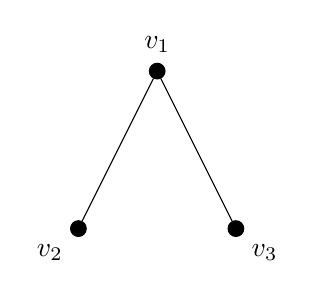
\begin{tikzpicture}
                    \node[circle, draw, fill=black, inner sep=2pt, label=above:\(v_1\)] (A) at (0, 1) {};
                    \node[circle, draw, fill=black, inner sep=2pt, label=below left:\(v_2\)] (B) at (-1, -1) {};
                    \node[circle, draw, fill=black, inner sep=2pt, label=below right:\(v_3\)] (C) at (1, -1) {};
                    \draw (A) -- (B);
                    \draw (A) -- (C);
                \end{tikzpicture}
            \end{center}

            \item \textbf{Graph 6:} \( (1, 0, 1) \), vertices \(v_1\),\(v_2\) and \(v_2\),\(v_3\) are connected, probability \( \bm{P = \left(\frac{1}{3}\right)^2 \cdot \frac{2}{3} = \frac{2}{27}} \).
            \begin{center}
                \begin{tikzpicture}
                    \node[circle, draw, fill=black, inner sep=2pt, label=above:\(v_1\)] (A) at (0, 1) {};
                    \node[circle, draw, fill=black, inner sep=2pt, label=below left:\(v_2\)] (B) at (-1, -1) {};
                    \node[circle, draw, fill=black, inner sep=2pt, label=below right:\(v_3\)] (C) at (1, -1) {};
                    \draw (A) -- (B);
                    \draw (B) -- (C);
                \end{tikzpicture}
            \end{center}

            \item \textbf{Graph 7:} \( (0, 1, 1) \), vertices \(v_1\),\(v_3\) and \(v_2\),\(v_3\) are connected, probability \( \bm{P = \left(\frac{1}{3}\right)^2 \cdot \frac{2}{3} = \frac{2}{27}} \).
            \begin{center}
                \begin{tikzpicture}
                    \node[circle, draw, fill=black, inner sep=2pt, label=above:\(v_1\)] (A) at (0, 1) {};
                    \node[circle, draw, fill=black, inner sep=2pt, label=below left:\(v_2\)] (B) at (-1, -1) {};
                    \node[circle, draw, fill=black, inner sep=2pt, label=below right:\(v_3\)] (C) at (1, -1) {};
                    \draw (A) -- (C);
                    \draw (B) -- (C);
                \end{tikzpicture}
            \end{center}

            \item \textbf{Graph 8:} \( (1, 1, 1) \), all vertices are connected, probability \( \bm{P = \left(\frac{1}{3}\right)^3 = \frac{1}{27}} \).
            \begin{center}
                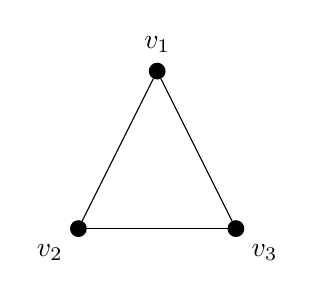
\begin{tikzpicture}
                    \node[circle, draw, fill=black, inner sep=2pt, label=above:\(v_1\)] (A) at (0, 1) {};
                    \node[circle, draw, fill=black, inner sep=2pt, label=below left:\(v_2\)] (B) at (-1, -1) {};
                    \node[circle, draw, fill=black, inner sep=2pt, label=below right:\(v_3\)] (C) at (1, -1) {};
                    \draw (A) -- (B);
                    \draw (A) -- (C);
                    \draw (B) -- (C);
                \end{tikzpicture}
            \end{center}
        \end{itemize}

        All the probabilities sum up to 1, as expected:
        \[
        \frac{8}{27} + 3 \cdot \frac{4}{27} + 3 \cdot \frac{2}{27} + \frac{1}{27} = 1.
        \]
    \end{solution}
    
    \question In \( G_{12,p} \) random graphs find a) the distribution and the average degree of
any vertex b) the distribution and the expectation of the number of edges.\droppoints

    \begin{solution}
        \begin{parts}
            \part The degree of a vertex \(v\) is the number of edges connected to that vertex. For n = 12 vertices each vertex can potentially have an edge to any of the other 11 vertices. For each of these 11 possible edges, there is a Bernoulli trial: either the edge exists (with probability p) or it does not exist (with probability 1 - p). The outcome of one trial does not affect the outcome of another trial. Thus, the degree of each vertex follows the \textbf{binomial distribution}.

            Let \(\bm{X} \) be the random variable that represents the degree of vertices in the \( G_{12,p} \) random graphs, then:

            \[
            \(\bm{X} \) \sim B\left(11, p\right)
            \]

            The average (expected) value of the random variable \(\bm{X} \) will be:

            \[
            \mathbb{E}[\(\bm{X} \)] = 11 \cdot p
            \]
            \part The number of edges in \( G_{12,p} \) is random and follows the \textbf{binomial distribution}. The reason why is first of all that the experiment for the creation of the random graphs (coin toss) is repeated for a fixed number of times (\( \binom{12}{2} = 66\), which is the amount of the edges). Also, every edge in the random  graph is a Bernoulli trial with success probability p, meaning the presence of an edge is a "success" and the absence of an edge is a "failure". Finally, the outcome of one trial does not affect the outcome of another trial.

            Let \(\bm{X} \) be the random variable that represents the amount of edges in the \( G_{12,p} \) random graphs, then:

            \[
            \(\bm{X} \) \sim B\left(66, p\right)
            \]

            The expected value of the random variable \(\bm{X} \) will be:

            \[
            \mathbb{E}[\(\bm{X} \)] = 66 \cdot p 
            \]
        \end{parts}
    \end{solution}
    
    \question Prove that if there is a real p, \( 0 \leq p \leq 1\), so that
    \[
    \Pr[M] \leq \binom{n}{k} p^{\binom{k}{2}} + \binom{n}{t} (1 - p)^{\binom{t}{2}},
    \]
    then the Ramsey number \( r(k, t) \) satisfies \( r(k, t) > n \).\droppoints
    
    \begin{solution}
        \begin{proof}
        The Ramsey number \( r(k, t) \) is the smallest integer \( n \) such that in any two-coloring of the edges of the complete graph on \( n \) vertices \( K_{n} \) by red and blue colors, either there is a red \( K_{k} \) or there is a blue \( K_{t} \). We aim to show that if the given inequality holds, then no random graph on \( n \) vertices guarantees such a structure, implying 
        \[
        \bm{r(k, t) > n}
        \]
        For this proof we will use the \textbf{Method of Positive Probability}. First, we construct a probability sample space by two-coloring at random every edge of \( K_{n} \), with probability \( p \) for red and \( 1 - p \) for blue, independently (for the edges). Let \( S_{k} \) be any fixed set of \( k \) vertices and \( S_{t} \) be any fixed set of \( t \) vertices. Then, for these sets we define the events \( M_{k} := \{ S_{k} \text{ forms a red } K_{k} \} \) and \( M_{t} := \{ S_{t} \text{ forms a blue } K_{t} \} \). In \( K_{k} \), we have \( \binom{k}{2} \) edges, and each one is colored red with probability \( p \). So the probability that all edges are red will be \( p \cdot p \cdot \cdots \cdot p \) (repeated \( \binom{k}{2} \) times), or 
    \[
    \boldsymbol{\Pr[M_k] = p^{\binom{k}{2}}}.
    \]
    In the same way, in \( K_{t} \), we have \( \binom{t}{2} \) edges, and each one is colored blue with probability \( 1 - p \). So the probability that all edges are blue will be \( (1 - p) \cdot (1 - p) \cdot \cdots \cdot (1 - p) \) (repeated \( \binom{t}{2} \) times), or 
    \[
    \boldsymbol{\Pr[M_t] = (1 - p)^{\binom{t}{2}}}.
    \]
    Next, we define the event \( M := \{ \exists \, \text{at least one red set of } k \text{ vertices or at least one} \right. \\
\left. \text{blue set of } t \text{ vertices} \right\} \).
 Using Boole's inequality, we have:
    \[
    \Pr[M] \leq \sum_{|S_k| = k} \Pr[M_k] + \sum_{|S_t| = t} \Pr[M_t]
    \]
    The total amount of \( S_{k} \) sets of size \( k \) is \( \binom{n}{k} \), since we want to find all the different ways we can choose \( k \) from \( n \) vertices. Similarly, the total amount of \( S_{t} \) sets of size \( t \) is \( \binom{n}{t} \). So, if we substitute in the inequality above, we have:
    \[
    \Pr[M] \leq \binom{n}{k} \Pr[M_k] + \binom{n}{t} \Pr[M_t] \Rightarrow
    \]
    \[
    \Pr[M] \leq \binom{n}{k} p^{\binom{k}{2}} + \binom{n}{t} (1 - p)^{\binom{t}{2}}.
    \]
    Finally, if \( \Pr[M] < 1 \), we require 
    \[
    \binom{n}{k} p^{\binom{k}{2}} + \binom{n}{t} (1 - p)^{\binom{t}{2}} < 1.
    \]
    If the above inequality holds, then 
    \[
    \bm{\Pr[\overline{M}] > 0}
    \]
    meaning there exists a graph with \( n \) vertices that avoids both:
    \begin{enumerate}
        \item A \( K_k \) with all red edges,
        \item A \( K_t \) with all blue edges.
    \end{enumerate}
    Hence, \( r(k, t) \) satisfies \( r(k, t) > n \).
    \end{proof}
    \end{solution}

    \question Prove that, for every integer $n$, there exists a coloring of the edges of the complete graph $K_n$ by two colors such that the total number of monochromatic $K_4$ subgraphs is at most 
\[
\binom{n}{4} \cdot 2^{-5}
\]\droppoints
    
    \begin{solution}
        \begin{proof}
        This proof will be based on \textbf{Linearity of Expectation}. First, we construct a probability sample space by two-coloring at random, equiprobably (for the two colors) and independently (for the edges) every edge of $K_n$. 
        
        Also, let \(\bm{X}\) be the random variable that denotes the total number of monochromatic $K_4$ subgraphs in $K_n$. We then have the subsets \( S\) of $K_n$ with 4 vertices and for each subset \( S\) of these we define the indicator r.v. \(\bm{X_S} \) such that:
        \[
        \bm{X_S} =
        \begin{cases} 
        1 & \text{if $S$ is monochromatic,} \\
        0 & \text{otherwise.}
        \end{cases}
        \]
        Since the indicator r.v. is a boolean, then in order to find the total amount of monochromatic $K_4$ subgraphs, i.e. the r.v. \(\bm{X}\), we can simply calculate the sum of the indicator r.v. over all subsets \( S\). Thus, we will have:
        \[
        \(\bm{X}\) = \sum_S \(\bm{X_S} \)
        \]
        We must note at this point that a $K_4$ complete graph has \( \binom{4}{2} = 6\) edges. To continue with the proof we must compute \( \mathbb{E}[X_S] \). A \( K_4 \) subgraph is monochromatic if all 6 of its edges are either red or blue. The probability that all 6 edges are red is \( \left(\frac{1}{2}\right)^6 \), and the probability that all 6 edges are blue is also \( \left(\frac{1}{2}\right)^6 \). Therefore:
        \[
        Pr[S \text{ is monochromatic}] = Pr[\(\bm{X_S} \)= 1] = \left(\frac{1}{2}\right)^6 + \left(\frac{1}{2}\right)^6 = 2 \cdot \left(\frac{1}{2}\right)^6 = \frac{1}{32} = 2^{-5}.
        \]
        Hence:
        
        \[
        \bm{\mathbb{E}[X_S] = Pr[\(\bm{X_S} \)= 1] = 2^{-5}}.
        \]
        Now, by Linearity of Expectation it holds true that:
        \[
        \mathbb{E}[\(\bm{X} \)] = \mathbb{E}[\sum_S \(\bm{X_S} \)] = \sum_S \mathbb{E}[\(\bm{X_S} \)]
        \]
        In total, the number of different subsets \( S\) of $K_4$ in $K_n$ will be \( \binom{n}{4}\), since we want to find all the different ways we can choose 4 from n vertices. If we substitute all the above in the previous equation we get the desired result:
        \[
        \mathbb{E}[\(\bm{X} \)] = \binom{n}{4} \cdot 2^{-5}
        \]
        Thus, there must exist at least one specific coloring of the edges of $K_n$ such that the total number of monochromatic $K_4$ subgraphs is at most the expected value \mathbb{E}[\(\bm{X} \)].
        \end{proof}
    \end{solution}

    \question Find the threshold probability for the existence, with high probability, of a $K_5$ in $G_{n,p}$.\droppoints
    
    \begin{solution}
    
    Let $A$ be the property of existence of $K_5$ cliques in $G_n,p$. Our goal is to find the threshold function $p_o(n)$ that activates property $A$ by using the \textbf{Second Moment Method}. In other words we must show that \[
\Delta^* = o(\mathbb{E}[X])
\] or equivalently
    \[
\frac{\Delta^*}{\mathbb{E}[X]} \to 0
\]

    To begin with, let $S$ be any fixed set of 5 vertices. We define the r.v. \(\bm{X} \) that counts the number of different cliques of size 5. We also define the indicator r.v. \(\bm{X_S} \) such that:
        \[
        \bm{X_S} =
        \begin{cases} 
        1 & \text{if $S$ is a clique,} \\
        0 & \text{otherwise.}
        \end{cases}
        \] 
    Since the indicator r.v. is a boolean, then in order to find the total amount of $K_5$ subgraphs, i.e. the r.v. \(\bm{X}\), we can simply calculate the sum of the indicator r.v. over all subsets \( S\) that have a size of 5. Thus, we will have:
        \[
\(\bm{X} \) = \sum_{S, \, |S|=5} \(\bm{X_S} \)
\]
    Each subset corresponds to a \( K_5 \) if all \( \binom{5}{2} = 10 \) edges exist. The probability that all 10 edges of a \( K_5 \) exist is Pr[S \text{ is a $K_5$ clique}] = Pr[\(\bm{X_S} \)= 1] = \( p^{10} \), since in \( G_{n,p} \) every edge exists independently with probability \( p \). So, we have:
    \[
        \bm{\mathbb{E}[\(\bm{X_S} \)] = Pr[\(\bm{X_S} \)= 1] = \( p^{10} \)}
    \]
    For the next step, again by Linearity of Expectation we have:
    \[
        \mathbb{E}[\(\bm{X} \)] = \mathbb{E}[\sum_{S, \, |S|=5} \(\bm{X_S} \)] = \sum_{S, \, |S|=5} \mathbb{E}[\(\bm{X_S} \)]
        \]
    In total, the number of different subsets \( S\) with size 5 will be \( \binom{n}{5}\), since we want to find all the different ways we can choose 5 from n vertices. If we substitute all the above in the previous equation we get:
    \[
\mathbb{E}[\(\bm{X} \)] = \binom{n}{5} \cdot p^{10} \sim {n^5} \cdot p^{10} \quad \text{(by approximation)}.
\]
    If we have \(\mathbb{E}[\bm{X}] = n^5 \cdot p^{10} \ll 1 \iff p \ll n^{-1/2} \), then property \( A \) won't hold true with high probability (w.h.p.), whereas if \( p \gg n^{-1/2} \), we have \( \mathbb{E}[X] \to \infty \), which means that the property exists w.h.p.
    
    We are done with the denominator of the fraction and now we must also compute the value of \(\bm{\Delta^* = \sum_{j \sim i} \mathbb{P}(A_j \mid A_i)}\). Firstly, we define the event $A_i$ as "set $S_i$ is a clique with size 5" and \( A_j \sim A_i \) if and only if $A_j$ and $A_i$ have common edges, but less than 5. $A_i$ and $A_j$ are not independent when \( i \neq j \), because they may share edges affecting their probabilities. So, \( A_j \sim A_i \) if and only if \( |S_i \cap S_j| \) = 2, 3, 4.

    \begin{itemize}
    \item \( |S_i \cap S_j| = 2 \): We have \( \binom{2}{2} =\) \textbf{1 common edge} and we are left with 9 more edges, so \( \mathbb{P}(A_j \mid A_i) = p^9 \). Also, there are \( \binom{5}{2} \cdot \binom{n-5}{3} = O(n^3) \) ways to choose \( S_j \), because we need to first choose the 2 common vertices from the 5, and then choose the remaining 3 vertices from the \( n-5 \) vertices in \( K_n \) to form the \( K_5 \) clique. Thus, \mathbf\[
\mathbf{\sum_{|S_i \cap S_j| = 2} \mathbb{P}(A_j \mid A_i)} = n^3 \cdot p^9
\]
    \item \( |S_i \cap S_j| = 3 \): We have \( \binom{3}{2} =\) \textbf{3 common edges} and we are left with 7 more edges, so \( \mathbb{P}(A_j \mid A_i) = p^7 \). Also, there are \( \binom{5}{3} \cdot \binom{n-5}{2} = O(n^2) \) ways to choose \( S_j \), because we need to first choose the 3 common vertices from the 5, and then choose the remaining 2 vertices from the \( n-5 \) vertices in \( K_n \) to form the \( K_5 \) clique. Thus, \mathbf\[
\mathbf{\sum_{|S_i \cap S_j| = 3} \mathbb{P}(A_j \mid A_i)} = n^2 \cdot p^7
\]
    \item \( |S_i \cap S_j| = 4 \): We have \( \binom{4}{2} =\) \textbf{6 common edges} and we are left with 4 more edges, so \( \mathbb{P}(A_j \mid A_i) = p^4 \). Also, there are \( \binom{5}{4} \cdot \binom{n-5}{1} = O(n) \) ways to choose \( S_j \), because we need to first choose the 4 common vertices from the 5, and then choose the remaining 1 vertex from the \( n-5 \) vertices in \( K_n \) to form the \( K_5 \) clique. Thus, \mathbf\[
\mathbf{\sum_{|S_i \cap S_j| = 4} \mathbb{P}(A_j \mid A_i)} = n \cdot p^4
\]
    \end{itemize}Finally, if we substitute all these we have:
    \[
    \Delta^* = \sum_{2 \leq |S_i \cap S_j| \leq 4} \mathbb{P}(A_j \mid A_i)\) = n^3 \cdot p^9 + n^2 \cdot p^7 + n \cdot p^4
    \]
    Now that we have calculated both quantities we compute the fraction \(\frac{\Delta^*}{\mathbb{E}[X]} = \frac{n^3 p^9 + n^2 p^7 + n p^4}{n^5 p^{10}} = \frac{1}{n^2 p} + \frac{1}{n^3 p^3} + \frac{1}{n^4 p^6}\). For \(\bm{p_0(n)=n^{-1/2}}\)  we will have:
    \[
    \mathbf{\frac{\Delta^*}{\mathbb{E}[X]} = \frac{1}{n^{3/2}} + \frac{1}{n^{9/2}} + \frac{1}{n^7} \to 0 \quad \text{as} \quad n \to \infty}
    \]
    \(\text{So, indeed, for that value of } p \text{ we have } \Delta^* = o(E[X]) \text{ and a } K_5 \text{ exists w.h.p.}\)
    \end{solution}

    \question Prove that any $k$-SAT formula in which no variable appears in more than 
$\frac{2^{k-2}}{k}$ clauses is satisfiable.\droppoints
    
    \begin{solution}
    \begin{proof}
    For this proof we will use the \textbf{Lov\'asz Local Lemma}. Let $n$ be the number of variables in the $k$-SAT formula: $x_1, x_2, \dots, x_n$.  
Each variable $x_i$ can take one of two truth values: \textit{True} or \textit{False}. The sample space $\Omega$ is the set of all possible truth assignments for the $n$ variables. Since each variable can take one of two values independently, the sample space will consist of all $2^n$ possible truth assignments.

Let there be \( m \) clauses \( C_1, C_2, \dots, C_m \) and \( A_i \) the event "clause \( C_i \) is unsatisfied.". The probability of this happening is:
\[
\bm{p=\Pr[A_i] = \frac{1}{2^k}}.
\]
since we want all \( k \) literals of the \(i\)-th clause to be \(False\), as it is in Conjunctive Normal Form (CNF). We aim to show that there exists a truth assignment such that no clause is unsatisfied, i.e., 
\[
\bm{\Pr\left[ \bigcap_{i=1}^{m} \overline{A_i} \right] > 0}.
\]
Then, we construct a dependency graph \( G \) with vertices corresponding to the clauses \( C_1, C_2, \dots, C_m \). Two vertices, i.e. clauses \( C_i \) and \( C_j \), are connected by an edge if they share at least one common variable $x_i$. This means that their satisfiability is not independent. Thus, the degree \( d \) of a clause \( C_i \) represents the number of other clauses that depend on \( C_i \), i.e., the number of clauses that share at least one variable with \( C_i \). To bound \( d \), we need to count all clauses \( C_j \) that share at least one variable with \( C_i \).

Each variable in \( C_i \) can each appear in at most $\frac{2^{k-2}}{k}-1$ other clauses. Thus, the total number of clauses \( C_j \) that depend on \( C_i \) is bounded by:
\[
\bm{d \leq k \cdot (\(\frac{2^{k-2}}{k} -1\))}.
\]
since each clause has \(k\) variables.

Next, to apply the symmetric version of the Lovász Local Lemma, we need to check if the following relationship holds true: \(\bm{4 \cdot d \cdot p < 1}\). If  we substitute \( p \) and \( d \) into the inequality we will have:
\[
4 \cdot \frac{1}{2^k} \cdot k \cdot (\(\frac{2^{k-2}}{k} -1\)) < 1\Leftrightarrow 4 \cdot \frac{2^{k-2}}{2^k} - 4 \cdot \frac{k}{2^k}< 1\Leftrightarrow 1 - \frac{2^{2-k}}{k}< 1\Leftrightarrow\frac{2^{2-k}}{k}>0
\]
Since \( \frac{2^{2-k}}{k} \) is positive for all \( k \geq 1 \) (in $k$-SAT the minimum value of $k$ is 1, which is the trivial case), then the inequality \(4 \cdot d \cdot p < 1\) holds true.

Therefore, we can conclude that \(\Pr\left[ \bigcap_{i=1}^{m} \overline{A_i} \right] > 0\) and by the Lovász Local Lemma, there exists a truth assignment such that no clause is unsatisfied. Hence, the k-SAT formula is satisfiable.
    \end{proof}
    \end{solution}

    \question Provide the details of the proof that Top-in-at-Random converges to a uniform distribution. Why this is important in the card shuffling context?\droppoints
    \begin{solution}
    
    Given a set of $n$ cards, let a Markov Chain whose states are all possible permutations of the cards ($n$!) and one step transition between states defined by the following card shuffling rule: \textbf{"place the top card to a random new position of the n possible ones"}. This rule is repeated for a sufficient amount of steps and the goal is to demonstrate that this method converges to a \textbf{uniform distribution} of cards. This means that as the number of shuffles tends to infinity, the probability of each permutation of the deck \textbf{converges to} \(\bm{\frac{1}{n!}}\), i.e. every permutation becomes equally likely.

    First, we define the set of all possible states $S$, where each state corresponds to a specific permutation of the deck. Since the position of the top card is chosen randomly from the $n$ possible positions, the probability of transitioning from any given state $S$ to any other state $S'$ is \(\bm{\frac{1}{n}}\). This holds true for all the transitions. Using this information we construct the $n!$ x $n!$ transition matrix $P$ for which we know the following:
    
    1) Each entry of the matrix is non-negative.

    2) Each row sums up to 1.

    3) Each column sums up to 1.

    These properties verify that the transition matrix is doubly stochastic and by the \textbf{Lemma in Lecture 9, slide 20} we know that this means that the stationary distribution \(\pi\) is \textbf{uniform}. 

    Finally, we now need to show that the Markov chain converges to the uniform distribution over time. The Markov chain is \textbf{ergodic}, \textbf{irreducible} and \textbf{aperiodic}, meaning that starting from any initial state, the chain will eventually visit all states with positive probability. This ensures that, after enough shuffling, the system will converge to the stationary distribution \(\pi\).

    The significance of the Top-in-at-Random shuffle is evident in card games, where ensuring fairness is crucial. If the shuffle is not truly random, some arrangements may occur more frequently, leading to bias and undermining the game's integrity. Another key application is determining the number of shuffles required to thoroughly randomize the deck and eliminate predictable patterns, a concept also known as mixing time. Additionally, in casinos or competitive card games, demonstrating that shuffling methods yield unbiased outcomes is vital for preserving trust and fairness.
    \end{solution}

    \question For a symmetric random walk on the following graph, (a) find the stationary distribution, if one exists, (b) estimate the expected time to move from $u$ to $v$, and (c) estimate the expected time between the successive visits to $u$. For all the above questions, use (i) the general Markov Chain methods of lecture 9, and (ii) the random walk tools of lecture 10.\droppoints
    \begin{solution}
    \begin{parts}
    \part
    \begin{minipage}{0.4\textwidth} % Width for the graph
        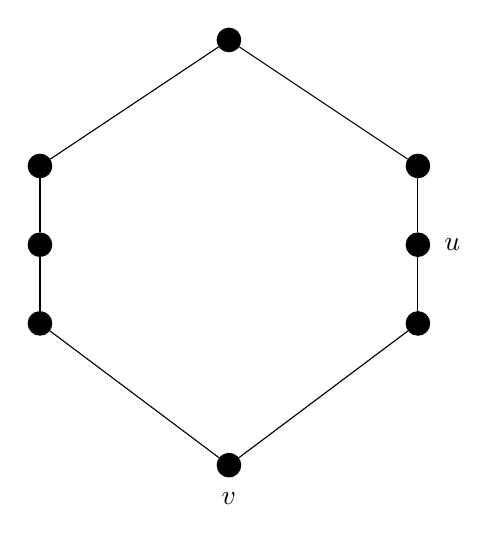
\begin{tikzpicture}[scale=2, every node/.style={circle, draw, fill=black, inner sep=3pt}] % Increased inner sep for larger nodes

        % Define the 8 nodes with coordinates and labels for u and v
        \node[circle, draw, fill=black, inner sep=3pt] (n1) at (0, 2) {};
        \node[circle, draw, fill=black, inner sep=3pt] (n2) at (-1.2, 1.2) {};
        \node[circle, draw, fill=black, inner sep=3pt] (n3) at (-1.2, 0.7) {};
        \node[circle, draw, fill=black, inner sep=3pt] (n4) at (-1.2, 0.2) {};
        \node[circle, draw, fill=black, inner sep=3pt, label=below:\(v\)] (n5) at (0, -0.7) {}; % Label for u
        \node[circle, draw, fill=black, inner sep=3pt] (n6) at (1.2, 0.2) {};
        \node[circle, draw, fill=black, inner sep=3pt, label=right:\(u\)] (n7) at (1.2, 0.7) {}; % Label for v
        \node[circle, draw, fill=black, inner sep=3pt] (n8) at (1.2, 1.2) {};

        % Draw edges to connect the nodes in a hexagon-like structure with vertical nodes
        \draw (n1) -- (n2);
        \draw (n2) -- (n3);
        \draw (n3) -- (n4);
        \draw (n4) -- (n5);
        \draw (n5) -- (n6);
        \draw (n6) -- (n7);
        \draw (n7) -- (n8);
        \draw (n8) -- (n1);
        \end{tikzpicture}
    \end{minipage}
    \begin{minipage}{0.55\textwidth} % Width for the text
        From the \textbf{Fundamental Theorem of Markov Chains}, an MC has a unique stationary distribution \( \pi \) \textbf{iff the MC is irreducible, finite, and aperiodic}.

        1) The given Markov Chain is \textbf{aperiodic} because the walker can move to any of its two neighbors (left or right) at each step, which means that we can have both even and odd-length paths. Thus, we can return to any node \( u \) in irregular intervals, and the GCD of possible return times is 1. This ensures the chain does not have a periodic structure.

        2) The given Markov Chain is \textbf{irreducible} because it is possible to reach any node from any other node in a finite number of steps, regardless of where the walker starts. Starting from any node \( u \), the walker can reach any other node \( v \) by moving along the cycle in either direction.
        \end{minipage}

        3) The given Markov Chain is \textbf{finite} because it has only 8 distinct nodes, meaning that it has 8 possible states (one for each node). Since there are a finite number of states, it satisfies the condition of having a finite state space.

        Since all the 3 conditions are satisfied, then we can conclude that a stationary distribution \( \pi \) exists for this MC. Also, using the \textbf{Lemma from Lecture 9, slide 21}, we know that in a symmetric random walk, the long-term probability of being at any node is proportional to its degree. Since every node in this graph has the same degree of 2 (each node is connected to two neighbors), the stationary distribution is \textbf{uniform} across all nodes. So: 
        \[
        \bm{\pi(x) = \frac{1}{8}, \quad \forall x \in \{1, 2, 3, \dots, 8\}}.
        \]
        Thus, the stationary distribution vector is:
        \[
        \bm{\pi = \left[ \frac{1}{8}, \frac{1}{8}, \frac{1}{8}, \frac{1}{8}, \frac{1}{8}, \frac{1}{8}, \frac{1}{8}, \frac{1}{8} \right]}.
        \]
        We also compute the transition matrix, which is:
        \[
        P = \begin{bmatrix}
        0 & \frac{1}{2} & 0 & 0 & 0 & 0 & 0 & \frac{1}{2} \\
        \frac{1}{2} & 0 & \frac{1}{2} & 0 & 0 & 0 & 0 & 0 \\
        0 & \frac{1}{2} & 0 & \frac{1}{2} & 0 & 0 & 0 & 0 \\
        0 & 0 & \frac{1}{2} & 0 & \frac{1}{2} & 0 & 0 & 0 \\
        0 & 0 & 0 & \frac{1}{2} & 0 & \frac{1}{2} & 0 & 0 \\
        0 & 0 & 0 & 0 & \frac{1}{2} & 0 & \frac{1}{2} & 0} \\
        0 & 0 & 0 & 0 & 0 & \frac{1}{2} & 0 & \frac{1}{2} \\
        \frac{1}{2} & 0 & 0 & 0 & 0 & 0 & \frac{1}{2} & 0
        \end{bmatrix}
        \]
        We can also see that this distribution \( \pi \)  verifies the following properties:
        
        1)\[
        \bm{P\cdot \pi = \left[ \frac{1}{8}, \frac{1}{8}, \frac{1}{8}, \frac{1}{8}, \frac{1}{8}, \frac{1}{8}, \frac{1}{8}, \frac{1}{8} \right] = \pi}
        \]
        2)\[\bm{\(\pi_1 + \pi_2 + ... + \pi_8 = 1\)}\]
        
        \part To estimate the expected time to move from $u$ to
    $v$ we need to calculate the hitting time $h_{uv}$. We will first calculate the value of the effective resistance between $u$ and $v$ as shown in \textbf{Lecture 10} for \textbf{Random Walks}. For $n$ vertices and distance $d$ between the two states, the resistance for the shortest path is $R_1=d$ and for the longest path is $R_2=n-d$. Since the two paths form parallel circuits we have:
    \[
    \bm{R_{uv} = \frac{d \cdot (n - d)}{d + (n-d)}\Rightarrow R_{uv} = \frac{d \cdot (n - d)}{n}}
    \]
    For \( n = 8 \) vertices and a distance \( d = 2 \) between $u$ and $v$, the value of the effective resistance becomes:
    \[
    \bm{R_{uv} = \frac{2 \cdot (8 - 2)}{8} = \frac{12}{8} = 1.5}
    \]
    We know that in a symmetric graph it holds true that \bm{$h_{uv}$=$h_{vu}$}. We also know from \textbf{Lemma in Slide 8} that the formula for the commute time is:
    \[
    \bm{CT_{uv} = 2m \cdot R_{uv}}
    \]
    Since we have $m$=8 edges then we get the following result:
    \[
    CT_{uv} = 2\cdot8 \cdot 1.5\Rightarrow \(h_{uv}\)+\(h_{vu}\)=24\Rightarrow 2\cdot \(h_{uv}\)=24\Rightarrow \bm{\(h_{uv}\)=12}
    \]
    Therefore, the expected time to move from $u$ to $v$ is \textbf{12 steps}.
    
        \part We will use the formulae for \textbf{Random Walks} from \textbf{Lemma 1 and Lemma 2 from Lecture 10, slide 4}. The expected time between successive visits to \( u \), denoted \( h_{uu} \), is:
        \[
        \bm{h_{uu} = \frac{1}{\pi_u}},
        \]
        where \( \pi_u \) is the stationary probability of vertex \( u \). Also, the stationary distribution of vertex \( u \) is:
    \[
    \bm{\pi_u = \frac{d(u)}{2m}},
    \]
    where:
    \begin{itemize}
        \item \( d(u) \): Degree of vertex \( u \).
        \item \( m \): Total number of edges in the graph.
    \end{itemize}
    In our case we have \( d(u) \) = 2 and \( m \) = 8, thus:
    \[
\bm{\pi_u = \frac{2}{2 \cdot 8} = \frac{1}{8} \Rightarrow h_{uu} = \frac{1}{\pi_u} = \frac{1}{1/8} \Rightarrow h_{uu} = 8}
\]
Therefore, the expected time between the successive visits to $u$ is \textbf{8 steps}.
        \end{parts}
    \end{solution}
\end{questions}
\end{document}
